\documentclass[9pt,twocolumn]{article}
\usepackage[margin=0.55in,columnsep=0.22in]{geometry}
\usepackage[T1]{fontenc}
\usepackage{lmodern}
\usepackage{microtype}
\usepackage{amsmath,amssymb,booktabs}
\usepackage{graphicx}
\usepackage{caption}
\usepackage{url}
\usepackage{enumitem}
\setlength{\parindent}{0pt}
\setlength{\parskip}{2pt}
\captionsetup{font=footnotesize,skip=3pt}
\setlist{nosep,leftmargin=*}
\title{\vspace{-1.5em}\Large\bfseries TABasco: Task-Aware Browser Tab Optimization using Reinforcement Learning}
\author{Aarussh Shrivastava (B24CM1001)\\IIT Jodhpur, CSL3090 Artificial Intelligence\\\url{https://github.com/Aarsussh/TABasco}}
\date{Assignment 2 -- October 2026}
\begin{document}
\maketitle
\vspace{-2em}
\begin{abstract}
TABasco is an original synthetic browser-tab management Markov decision process (MDP) with a reward-trained Deep Q-Network (DQN) \cite{mnih}. In an initial soft-budget evaluation, DQN earned higher composite return while exceeding the memory budget more often. Increasing the memory penalty reduced but did not remove violations, so a separate constraint-aware transition variant was trained. On the previously examined 60-session evaluation block, it maintained the simulator's active-memory invariant. DQN had higher composite return than suspension baselines, although those baselines retained a larger fraction of useful revisits. These results characterize this simulator and reward, not a real browser.
\end{abstract}

\section{MDP and simulator}
For $N=12$ slots, state $s_t\in\mathbb{R}^{8N+5}$ is a fixed 101-value vector. Each slot contains occupied and active indicators, normalized memory size, recency, frequency, current-task match, estimated revisit probability, and unsaved-work risk. Five global fields encode active-memory/budget ratio, task, remaining horizon, elapsed fraction, and occupancy. Tab sizes are sampled from 0.45--1.35 synthetic units. Task switches, arrivals, revisits, and expiration evolve stochastically; revisit probability depends on age, frequency, and task affinity.

There are $3N+1=37$ discrete actions. Action $3i+o$ applies KEEP, SUSPEND, or CLOSE to slot $i$; the last action is WAIT. KEEP is valid for occupied tabs and restores a suspended tab; KEEP on an active tab is a charged no-op. SUSPEND requires an active tab; CLOSE requires occupancy. Empty-slot actions and redundant suspension are invalid. WAIT is always valid. One management action advances one time step; episodes end at a fixed 120-step horizon rather than when tabs are gone.

Only active tabs consume budget $B=8$; suspended tabs retain metadata at zero active-memory cost. A suspended revisit restores the tab and incurs restoration cost. Closed pages retain 30-step recovery history; a recovery incurs restoration and lost-work cost. Expiration charges risk-weighted loss and retains history. The agent observes each slot's state and a probability estimate, not future random events.

The soft-budget reward is the negative sum of nonnegative costs:
\begin{align*}
r_t=-[&c_m\max(0,M_t-B)+C_{\rm restore}+1.2C_{\rm lost}\\
&+0.45C_{\rm disrupt}+C_{\rm action}+C_{\rm deferred}],
\end{align*}
where $c_m=1$ in the selected configuration, restoration has multiplier 0.8, and ordinary action/WAIT and invalid-action costs are 0.035 and 0.12. Deferred environment events cost 0.25 in constrained mode. Every step exposes component values; the logged cost sum equals $-r_t$. There is no tab-count bonus or terminal reward.

\section{Constraint-aware variant}
The penalty sweep (coefficients 1, 3, 5; two fresh training seeds each) left 11.18\%, 9.89\%, and 8.59\% of validation steps over budget, respectively. Stronger penalty alone was insufficient. The selected variant makes active memory a transition invariant: initial overflow tabs start suspended; infeasible KEEP restores are masked; a suspended revisit that cannot fit stays suspended; closed recovery that cannot fit remains in history; and an arrival that cannot fit is declined, not queued. Deferrals incur 0.25 cost and can be retried only through future stochastic revisit/recovery events. Every transition asserts $M_t\leq B$, including after automatic events. This is an environment-enforced guarantee in the defined simulator, not a learned guarantee or real-process memory bound.

\section{Learning and comparison}
The DQN has a 101--128--128--37 ReLU MLP, Adam ($10^{-3}$), replay capacity 50,000, batch 64, discount 0.97, Huber loss, gradient clipping at 10, and target update every 500 learner updates. Epsilon decays 1.0 to 0.05 over 20,000 decisions. The same state-derived action mask is used for exploration, greedy selection, and replay bootstrap values. Two agents were initialized independently (seeds 3090, 4090) and trained on CPU for 250 episodes of up to 120 steps.

LRU suspends the eligible active tab with oldest last visit; LFU selects least frequency then oldest; Random samples uniformly from that same active-tab suspension set. Each waits if the set is empty. These are independent evaluation policies, not training labels \cite{sutton}. Policies share each episode's initial condition and event seed. DQN is greedy at evaluation. The selected checkpoint block was evaluated on seeds 91000--91059. This block was examined in earlier project analysis; it is a reused, previously examined evaluation, not a newly untouched test set.

\clearpage
\section{Measured results}
Table~\ref{tab:results} reports mean return and scenario SD over 60 episodes. Every policy had zero violation steps and invalid actions under the constrained transition rule. Mean active memory ranged from 5.50--5.80 for DQN and 1.18--1.25 for baselines, below budget 8. DQN useful-revisit success was 0.824 and 0.849; LRU, LFU, and Random achieved 0.886, 0.886, and 0.887. Thus the higher composite return coexists with fewer useful revisits for DQN.

\begin{table}[ht]
\centering\scriptsize
\caption{Previously examined evaluation block (60 shared seeds). Return is mean $\pm$ scenario SD.}
\label{tab:results}
\begin{tabular}{lrrrr}
\toprule Policy & Return & Mem. & Useful & Viol.\\
\midrule
DQN 3090 & $-21.70\pm4.51$ & 5.50 & .824 & 0\\
DQN 4090 & $-16.31\pm3.52$ & 5.80 & .849 & 0\\
LRU & $-58.38\pm4.67$ & 1.18 & .886 & 0\\
LFU & $-58.43\pm4.67$ & 1.18 & .886 & 0\\
Random & $-58.55\pm4.62$ & 1.25 & .887 & 0\\
\bottomrule
\end{tabular}
\end{table}

The aggregate reward components explain the return gap: DQN restoration costs were 5.69 and 4.37, disruption 3.67 and 2.07; LRU/LFU/Random incurred 16.32--16.35 restoration and 36.17--36.30 disruption. DQN deferred-event costs were 1.41 and 1.34, while baselines rarely deferred. Mean lost work was 6.73 and 4.33 for DQN versus about 1.69 for baselines. DQN's improvement is therefore a reward-weighted tradeoff, not universal superiority. Figure~\ref{fig:return} gives return variability; Figure~\ref{fig:memory} shows active-memory use.

\begin{figure}[ht]
\centering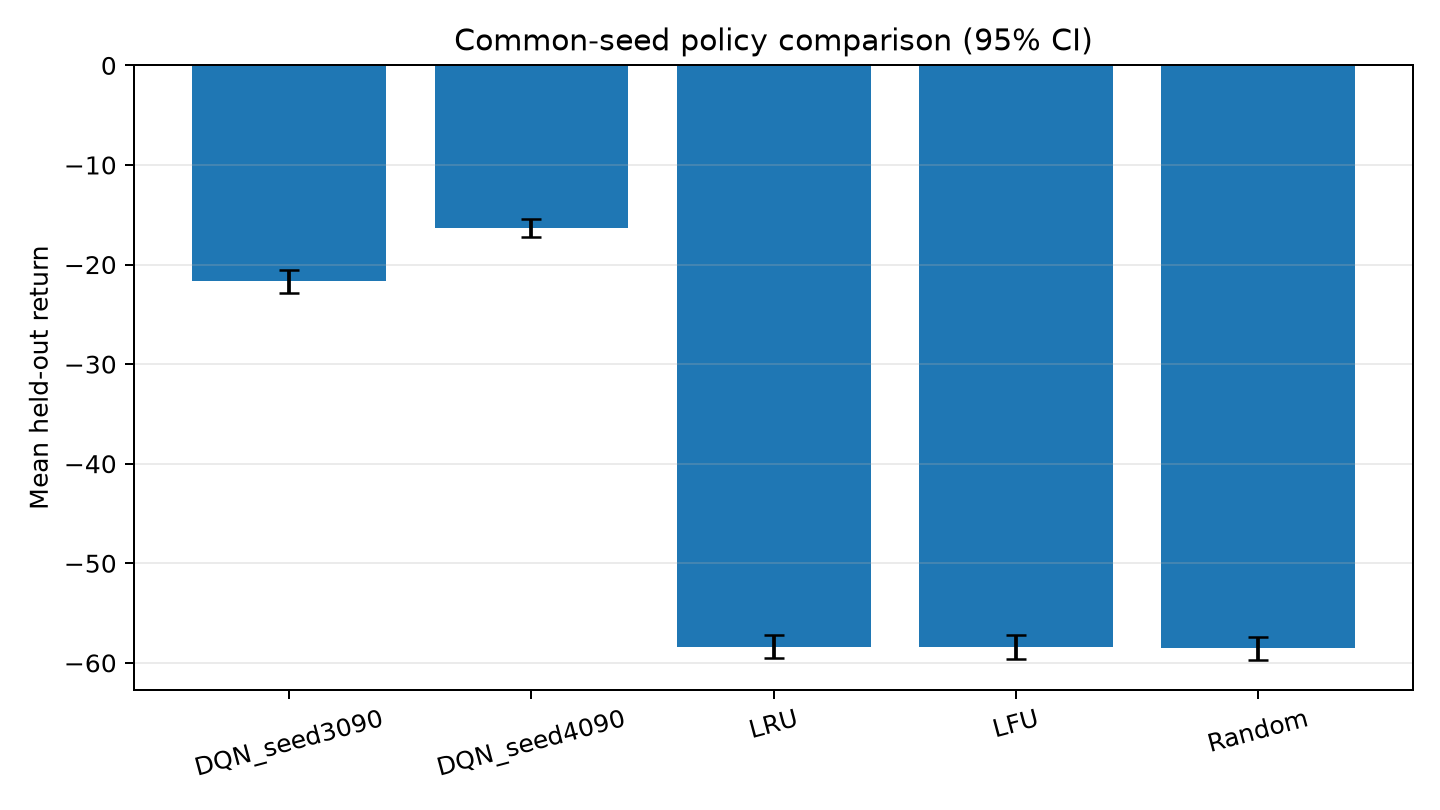
\includegraphics[width=\columnwidth]{../results/sensitivity/plots/heldout/return_comparison.png}
\caption{Mean return and 95\% scenario confidence intervals.}
\label{fig:return}
\end{figure}
\begin{figure}[ht]
\centering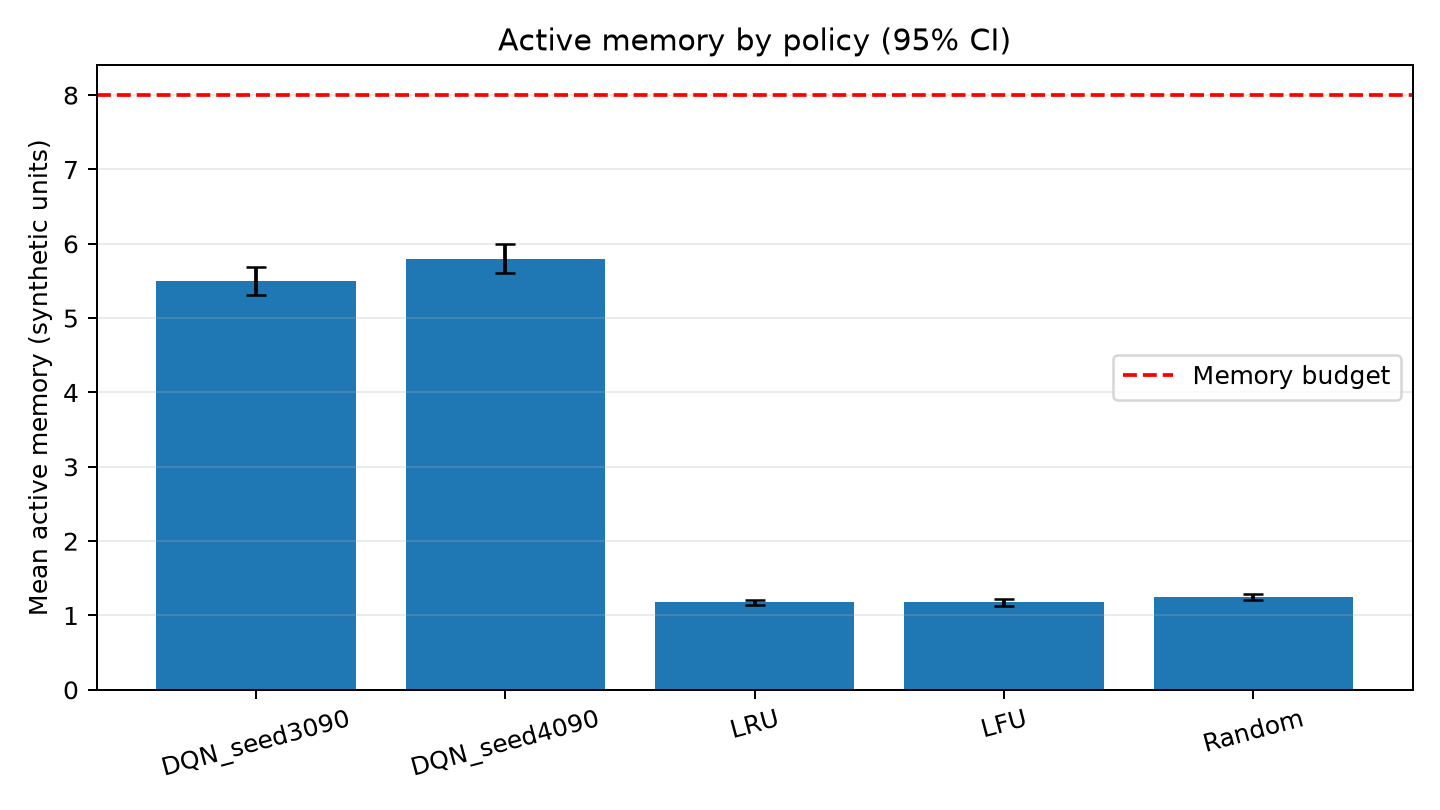
\includegraphics[width=\columnwidth]{../results/sensitivity/plots/heldout/memory_comparison.png}
\caption{Mean active memory and 95\% scenario confidence intervals; dashed line is budget 8.}
\label{fig:memory}
\end{figure}

\section{Validation and limitations}
A later reward-weight validation study compared current weights with restoration, lost-work, disruption, and balanced candidates. The strongest average candidate effect was only descriptive: lowering disruption weight to 0.35 changed canonical paired return by +2.43 for DQN seed 3090 (95\% scenario CI +0.26 to +4.59) and -1.47 for seed 4090 (-3.43 to +0.49), mean +0.48 across two training seeds. Useful-revisit success also fell from .820/.834 to .797/.802. The direction reversed across seeds and uncertainty remained; the current model was retained. The previously examined evaluation block was not used to choose this candidate.

V1's unmasked action selection and bootstrap, inconsistent invalid/no-op handling, early all-tabs-closed termination, and uncharged loss at expiration were corrected in subsequent versions. Current constraints are environment-enforced; they do not establish what a deployed tab manager should do when users return to pages that cannot fit. All workload probabilities and memory units are synthetic. Two training seeds are insufficient to characterize training variability; the scenario intervals condition on the fixed learned policies. Future work needs more seeds, measured browsing traces, calibrated memory, and user-valued deferral/recovery costs.

\clearpage
\onecolumn
\begin{thebibliography}{9}
\bibitem{mnih} V. Mnih et al., ``Human-level control through deep reinforcement learning,'' \emph{Nature}, vol. 518, pp. 529--533, 2015. doi: \url{https://doi.org/10.1038/nature14236}.
\bibitem{sutton} R. S. Sutton and A. G. Barto, \emph{Reinforcement Learning: An Introduction}, 2nd ed. MIT Press, 2018.
\end{thebibliography}
\end{document}
